\subsection{SharedLib}
I det følgende afsnit kan der læses om integrationstest for \gls{SL}.

\textbf{Introduktion}\\
Integrationstests for \gls{SL} blev ikke udført med andre delsystemer da dette var et bibliotek, det blev besluttet at dette bibliotek skulle have integrationstests for sig selv så der på alle tidspunkter kunne være sikkerhed om at det ikke var \gls{SL} der fejlede.\\

\textbf{Testdetaljer}\\
Testene er foretaget ved hjælp af NUnit og NSubstitute. For at finde ud af, hvilke klasser der skulle testes sammen er der udarbejdet et dependency tree, som kan ses på figur \ref{fig:SL-dependencies}.\\


\textbf{Beskrivelse af integrationstest}\\
Da designet af \gls{SL} havde gjort bibliotekets struktur meget overskuelig, var det også forholdsvis simpelt at teste, dog krævede det at der blev håndkodet to fakes. En der skulle agerer marshaller og en der skulle agere command. 

Testene blev udført ud fra "Top-down" metoden hvor der tages udgangspunkt i roden af programmet og først testes alle dennes forbindelser til laget under og derefter testes herfra og til næste lag indtil hele programmet er gennemtestet. 

Dette betød for \gls{SL}\footnote{For overblik over \gls{SL}'s protokol struktur, se da figur \ref{fig:overklasseSL} på side \pageref{fig:overklasseSL}} at de første tests der skulle udføres var fra Protocol klassen og så til XmlMarshaller for at se om funktionskaldene encode og decode også blev kaldt videre på den korrekte marshaller\footnote{Hvis den korrekte marshaller bliver kaldt er indholdet læst korrekt, da XmlMarshaller finder dette på baggrund af kommandonavnet.}.

Dernæst skulle der testes fra Protocol klassen og ned til nederste lag, altså selve marshallerne, og det blev her testet om de korrekte data, i dette tilfælde oprettelse af et produkt, blev encoded til en korrekt formateret XML string og derefter også om de korrekte data fra en XML string på decoded til et korrekt CreateProductCmd objekt.

\textbf{Dependency tree}
\begin{figure}[H]
	\centering
	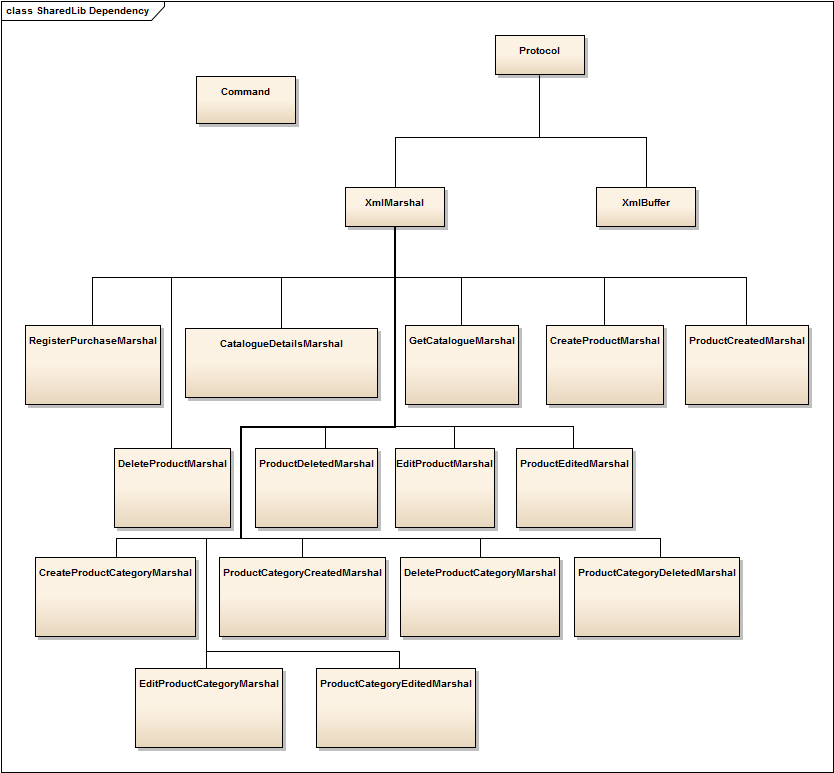
\includegraphics[width=1\textwidth]{Test/SharedLib/Integrationstest/SharedLib_Dependency.png}
	\caption{Dependency tree for \gls{SL}}
	\label{fig:SL-dependencies}
\end{figure}

